\subsection{Summary of Results (7+8 TeV)}

%%%%%%%%%%%%%%%%%%%%%%%%%%%%%%
\begin{figure}[!hbtp]
\centering
\subfigure[SM Higgs (BDT shape-based) 7 TeV ]{
\centering
\label{subfig:sm_shape_7tev}
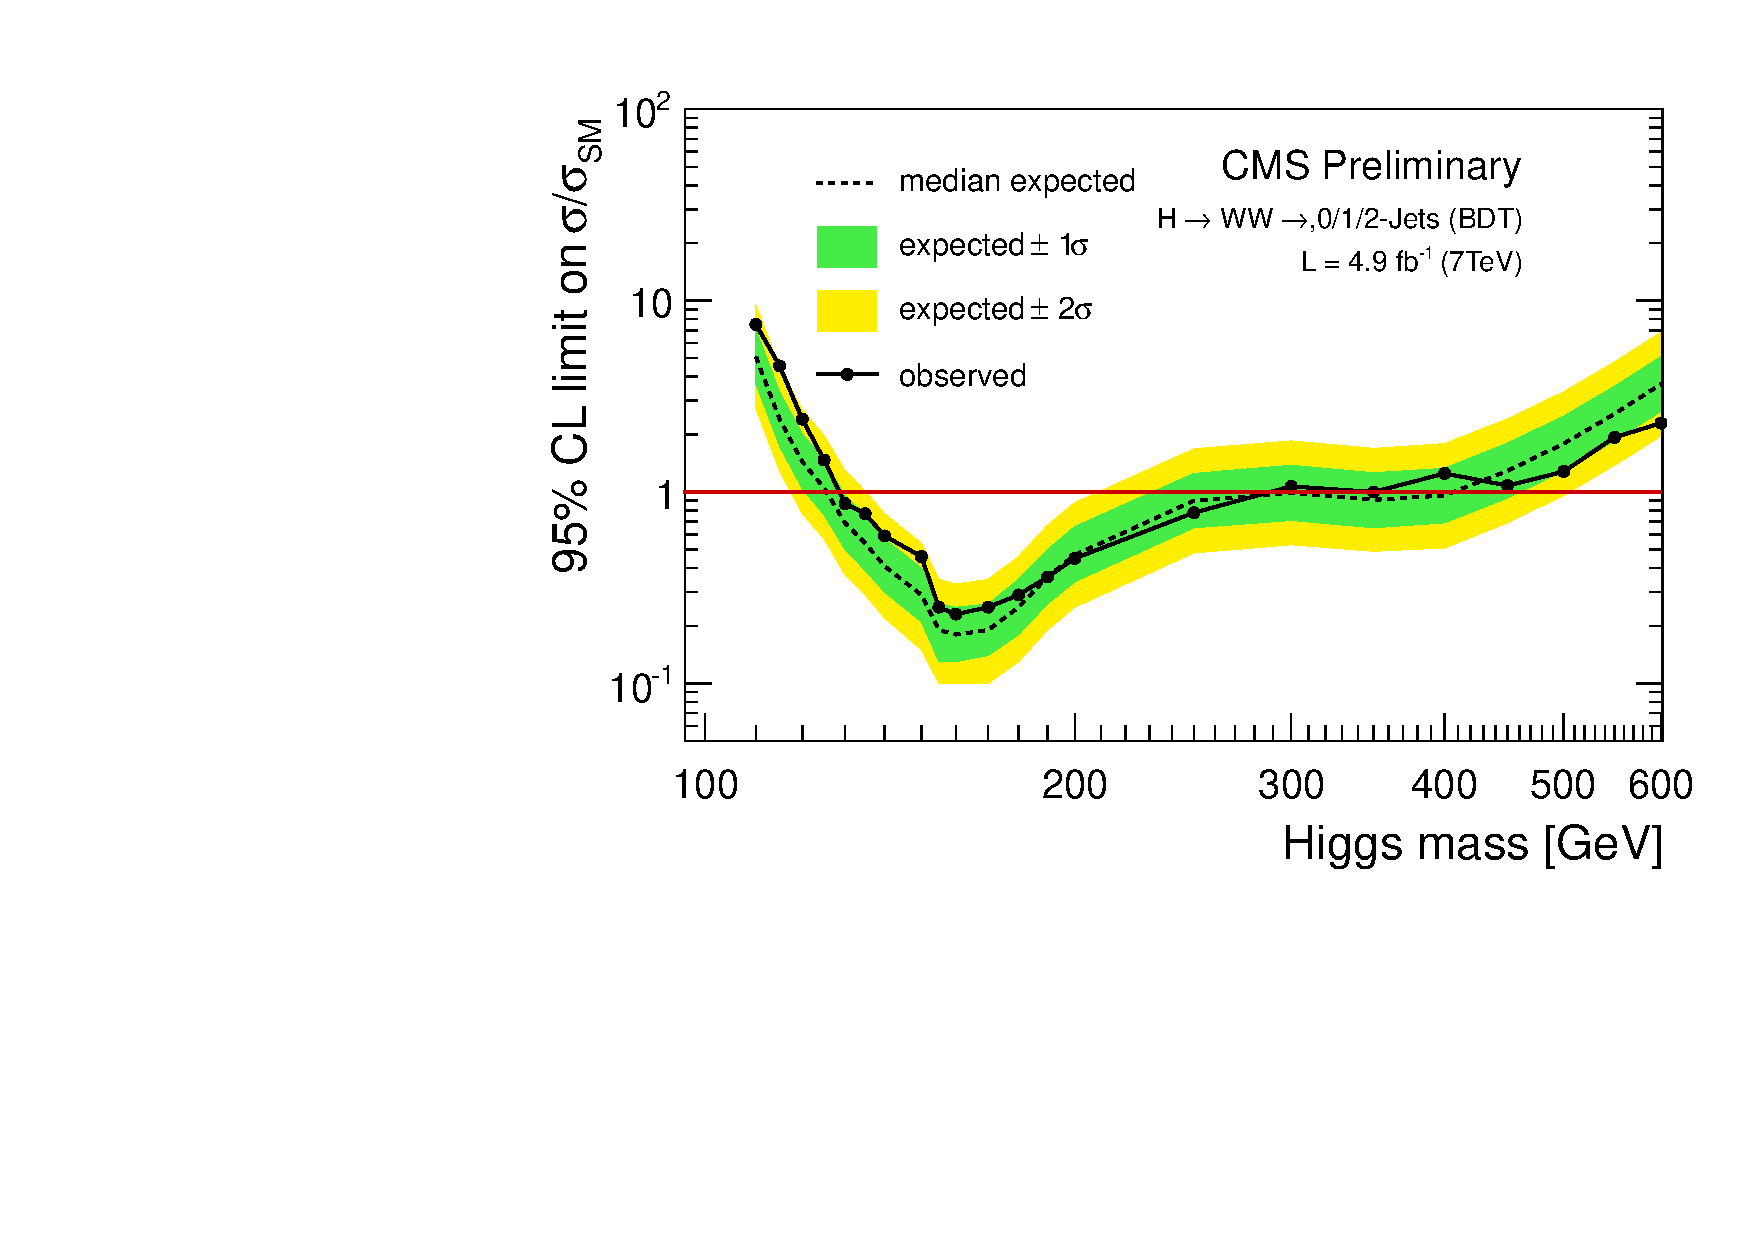
\includegraphics[width=.45\textwidth]{figures/limits_nj_shape_7TeV-CLs-asymptotic_log.pdf}}
\centering
\subfigure[SM Higgs (shape-based) 8 TeV ]{
\centering
\label{subfig:sm_shape_8tev}
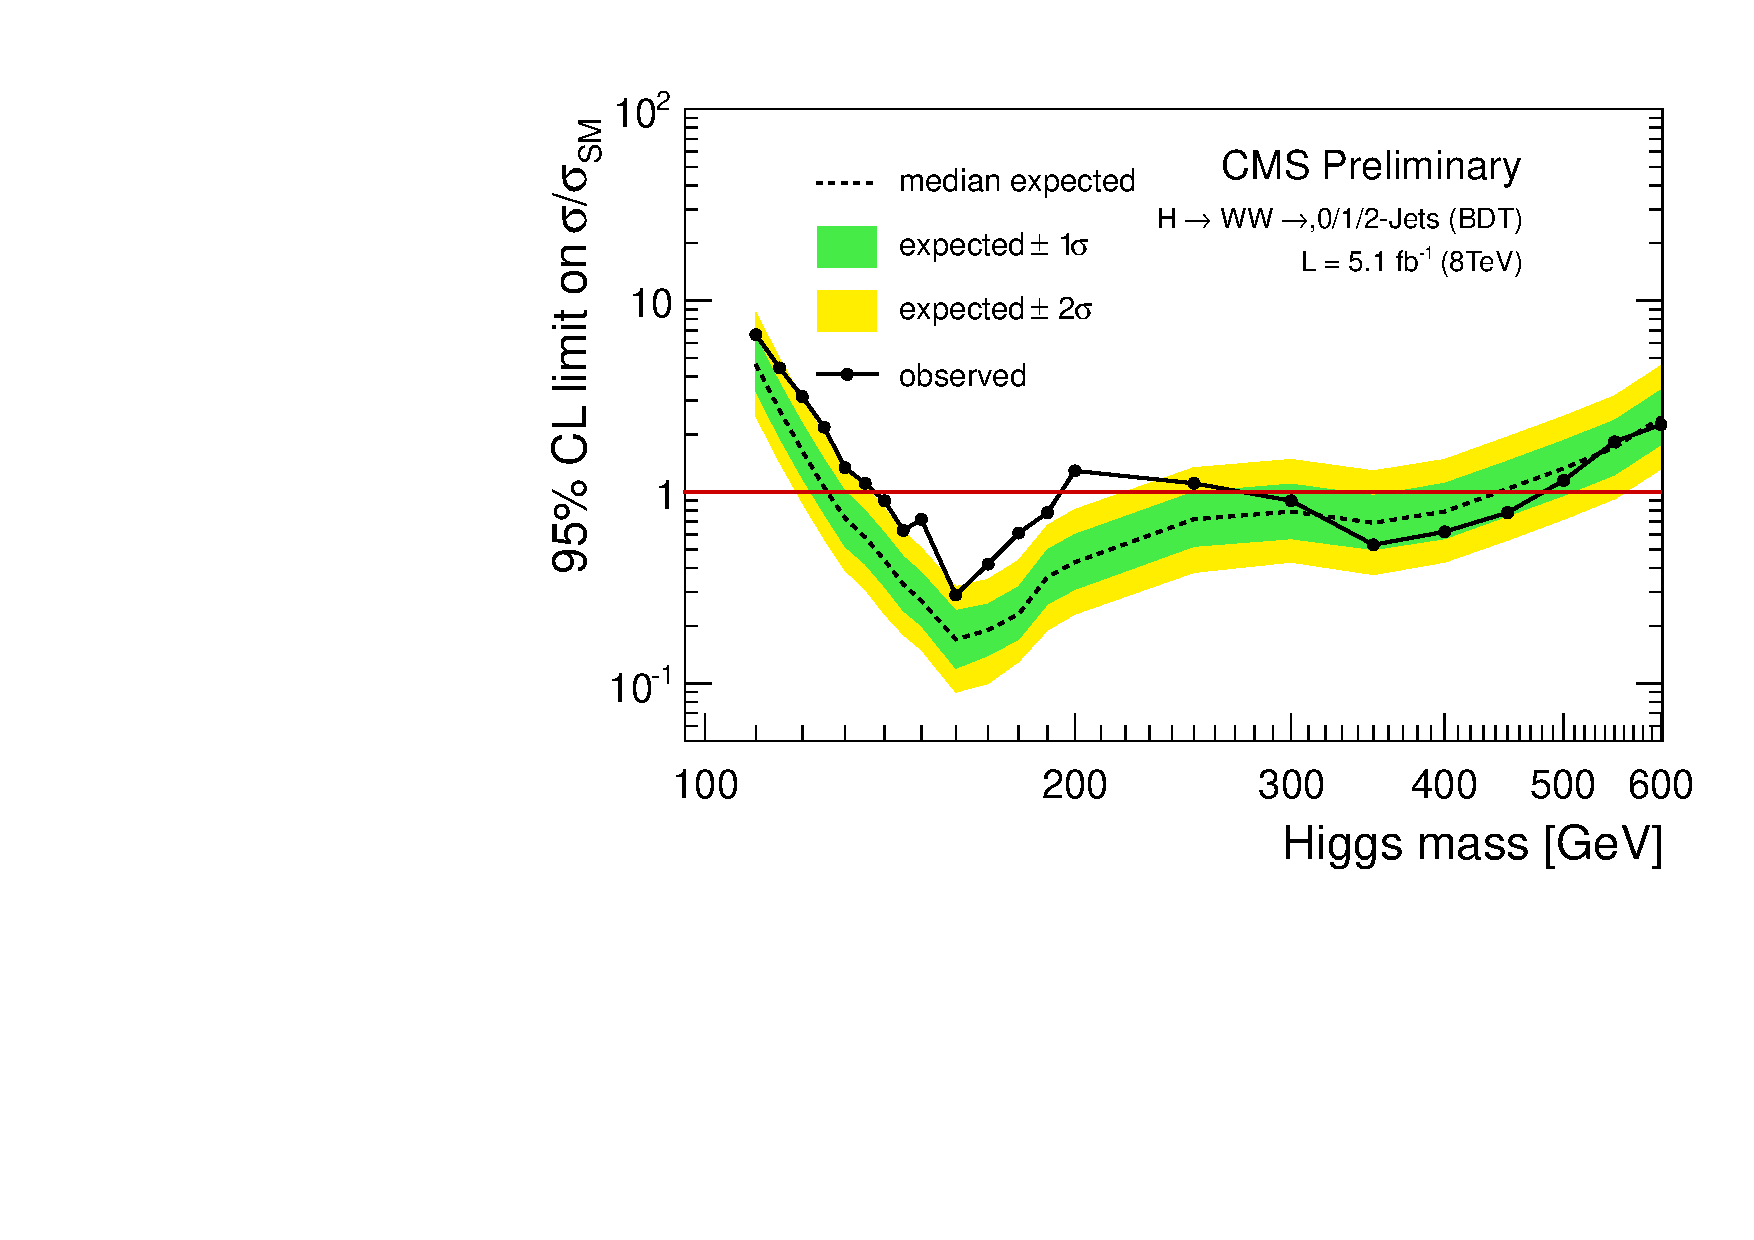
\includegraphics[width=.45\textwidth]{figures/limits_nj_shape_8TeV-CLs-asymptotic_log.pdf}} \\
\subfigure[SM Higgs (shape-based) 7+8 TeV ]{
\centering
\label{subfig:sm_shape_comb}
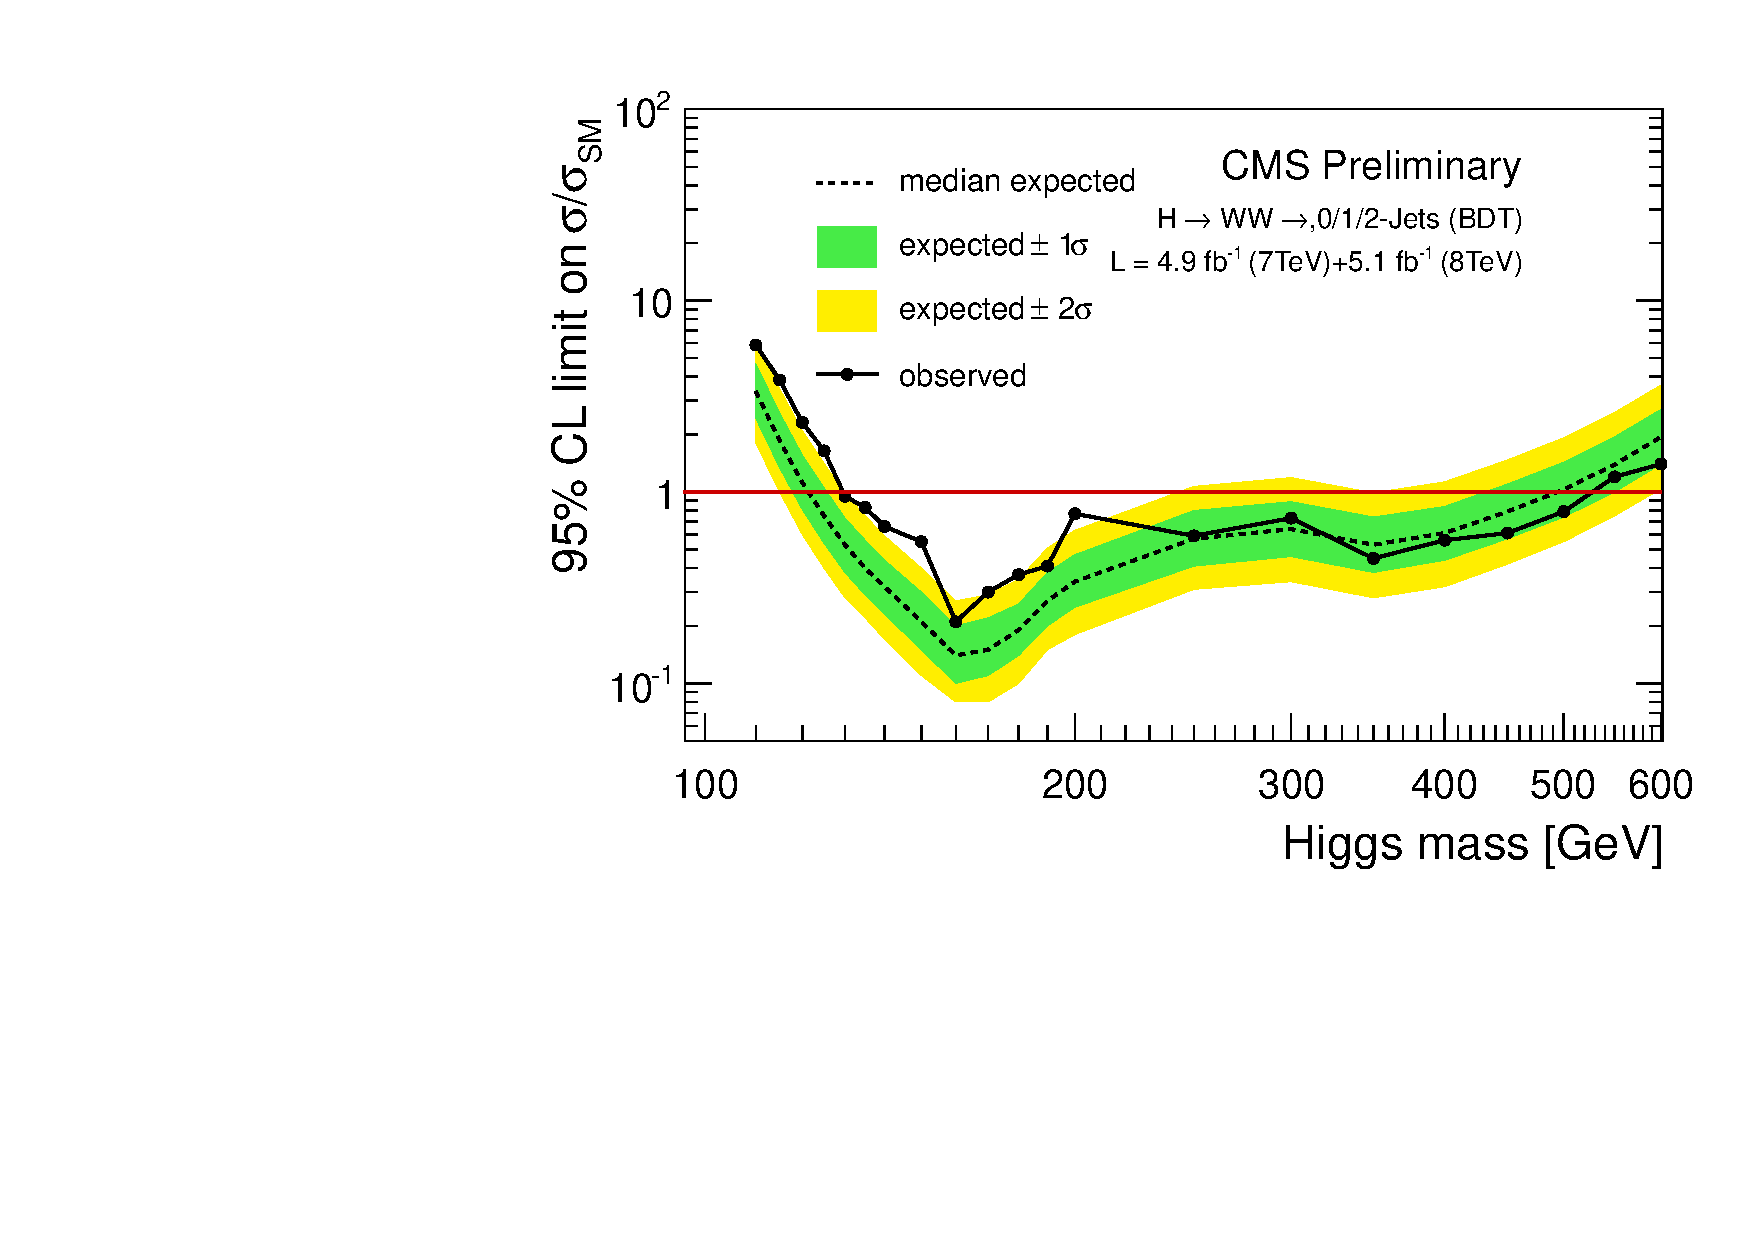
\includegraphics[width=.45\textwidth]{figures/limits_nj_shape-CLs-asymptotic_log.pdf}} \\ 
\label{fig:uls_shape}
\caption{Expected and observed upper limits for SM Higgs using the
  {\bf shape-based} analysis using 7 TeV, 8 TeV and combined data.}
\end{figure}

%%%%%%%%%%%%%%%%%%%%%%%%%%%%%%%%%%%%%%%%%%%%%%%%%%%%%%%%%%%%
\begin{table}[hbp!]
\begin{center}
\begin{tabular}{c c c c c}
\hline
\vspace{-3mm} && \\
 Higgs Mass & Observed  & Median expected & Expected range for 68\% & Expected range for 95\%   \\
\hline
\vspace{-3mm} && \\
110 & 7.51 & 5.09 & [3.67, 7.08] & [2.73, 9.49] \\
115 & 4.56 & 2.40 & [1.73, 3.33] & [1.29, 4.47] \\
120 & 2.40 & 1.44 & [1.04, 2.01] & [0.77, 2.69] \\
125 & 1.47 & 1.05 & [0.76, 1.47] & [0.57, 1.97] \\
130 & 0.87 & 0.69 & [0.50, 0.96] & [0.37, 1.29] \\
135 & 0.77 & 0.54 & [0.39, 0.76] & [0.29, 1.01] \\
140 & 0.59 & 0.41 & [0.30, 0.57] & [0.22, 0.77] \\
150 & 0.14 & 0.29 & [0.21, 0.40] & [0.15, 0.54] \\
160 & 0.23 & 0.18 & [0.13, 0.25] & [0.10, 0.33] \\
170 & 0.25 & 0.19 & [0.14, 0.26] & [0.10, 0.35] \\
180 & 0.29 & 0.25 & [0.18, 0.35] & [0.13, 0.46] \\
190 & 0.36 & 0.36 & [0.26, 0.50] & [0.19, 0.67] \\
200 & 0.45 & 0.47 & [0.34, 0.66] & [0.25, 0.88] \\
250 & 0.78 & 0.90 & [0.65, 1.25] & [0.48, 1.68] \\
300 & 1.07 & 0.99 & [0.71, 1.38] & [0.53, 1.85] \\
350 & 1.00 & 0.91 & [0.65, 1.26] & [0.49, 1.69] \\
400 & 1.25 & 0.96 & [0.69, 1.33] & [0.51, 1.79] \\
450 & 1.08 & 1.29 & [0.93, 1.80] & [0.69, 2.41] \\
500 & 1.28 & 1.79 & [1.29, 2.49] & [0.96, 3.34] \\
550 & 1.93 & 2.56 & [1.85, 3.57] & [1.38, 4.78] \\
600 & 2.29 & 3.66 & [2.64, 5.09] & [1.96, 6.83] \\
\hline
\end{tabular}
\caption{Expected and observed upper limits for SM Higgs using the
  {\bf shape-based} analysis, corresponding to $\intlumiSevenTeV$ at 7 TeV. }
\label{tab:shapebase_uls_7tev}
\end{center}
%\end{table}
%%%%%%%%%%%%%%%%%%%%%%%%%%%%%%
%\begin{table}[hbp!]
\begin{center}
\begin{tabular}{c c c c c}
\hline
\vspace{-3mm} && \\
 Higgs Mass & Observed  & Median expected & Expected range for 68\% & Expected range for 95\%   \\
\vspace{-3mm} && \\
\hline
110 & 6.64 & 4.64 & [3.34, 6.45] & [2.49, 8.65] \\
115 & 4.45 & 2.67 & [1.92, 3.71] & [1.43, 4.98] \\
120 & 3.15 & 1.64 & [1.18, 2.28] & [0.88, 3.06] \\
125 & 2.18 & 1.06 & [0.77, 1.48] & [0.57, 1.99] \\
130 & 1.34 & 0.73 & [0.52, 1.01] & [0.39, 1.35] \\
135 & 1.11 & 0.58 & [0.42, 0.80] & [0.31, 1.08] \\
140 & 0.90 & 0.44 & [0.32, 0.61] & [0.23, 0.82] \\
145 & 0.63 & 0.33 & [0.24, 0.46] & [0.18, 0.62] \\
150 & 0.72 & 0.27 & [0.20, 0.38] & [0.15, 0.51] \\
160 & 0.29 & 0.17 & [0.12, 0.24] & [0.09, 0.32] \\
170 & 0.42 & 0.19 & [0.14, 0.26] & [0.10, 0.35] \\
180 & 0.61 & 0.23 & [0.17, 0.32] & [0.13, 0.44] \\
190 & 0.78 & 0.36 & [0.26, 0.50] & [0.19, 0.67] \\
200 & 1.29 & 0.43 & [0.31, 0.60] & [0.23, 0.81] \\
% 200 & 0.34 & 0.43 & [0.31, 0.60] & [0.23, 0.81] \\ rMax = 50 for observed
250 & 1.11 & 0.72 & [0.52, 1.00] & [0.38, 1.34] \\
300 & 0.90 & 0.79 & [0.57, 1.10] & [0.43, 1.48] \\
350 & 0.53 & 0.69 & [0.50, 0.96] & [0.37, 1.29] \\
400 & 0.62 & 0.79 & [0.57, 1.11] & [0.43, 1.48] \\
450 & 0.78 & 1.04 & [0.75, 1.45] & [0.56, 1.94] \\
500 & 1.15 & 1.33 & [0.96, 1.86] & [0.72, 2.49] \\
550 & 1.83 & 1.71 & [1.23, 2.37] & [0.92, 3.18] \\
600 & 2.25 & 2.45 & [1.77, 3.41] & [1.32, 4.57] \\
\hline
\end{tabular}
\caption{Expected and observed upper limits for SM Higgs using the
  {\bf shape-based} analysis with \intlumiEightTeV\ of data at 8 TeV.}
\label{tab:shapebase_uls_8tev}
\end{center}
\end{table}
%%%%%%%%%%%%%%%%%%%%%%%%%%%%%%
\begin{table}[hbp!]
\begin{center}
\begin{tabular}{c c c c c}
\hline
\vspace{-3mm} && \\
 Higgs Mass & Observed  & Median expected & Expected range for 68\% & Expected range for 95\%   \\
\hline
110 & 5.86 & 3.35 & [2.42, 4.67] & [1.80, 6.25] \\
115 & 3.85 & 1.86 & [1.34, 2.59] & [1.00, 3.47] \\
120 & 2.31 & 1.12 & [0.81, 1.56] & [0.60, 2.09] \\
125 & 1.64 & 0.75 & [0.54, 1.05] & [0.40, 1.41] \\
130 & 0.95 & 0.53 & [0.38, 0.73] & [0.28, 0.98] \\
135 & 0.83 & 0.40 & [0.29, 0.56] & [0.22, 0.75] \\
140 & 0.66 & 0.32 & [0.23, 0.44] & [0.17, 0.59] \\
150 & 0.55 & 0.21 & [0.15, 0.30] & [0.11, 0.40] \\
160 & 0.21 & 0.14 & [0.10, 0.20] & [0.08, 0.27] \\
170 & 0.30 & 0.15 & [0.11, 0.22] & [0.08, 0.29] \\
180 & 0.37 & 0.19 & [0.14, 0.26] & [0.10, 0.35] \\
190 & 0.41 & 0.27 & [0.20, 0.38] & [0.15, 0.51] \\
200 & 0.77 & 0.34 & [0.25, 0.47] & [0.18, 0.63] \\
250 & 0.59 & 0.57 & [0.41, 0.80] & [0.31, 1.07] \\
300 & 0.73 & 0.64 & [0.46, 0.89] & [0.34, 1.19] \\
350 & 0.45 & 0.53 & [0.38, 0.74] & [0.28, 0.99] \\
400 & 0.56 & 0.61 & [0.44, 0.84] & [0.32, 1.13] \\
450 & 0.61 & 0.79 & [0.57, 1.10] & [0.42, 1.47] \\
500 & 0.79 & 1.03 & [0.74, 1.43] & [0.55, 1.92] \\
550 & 1.20 & 1.39 & [1.00, 1.94] & [0.75, 2.60] \\
600 & 1.40 & 1.94 & [1.40, 2.70] & [1.04, 3.62] \\
\hline
\end{tabular}
\caption{Expected and observed upper limits for SM Higgs using the
  {\bf shape-based} analysis, corresponding to $\intlumiSevenTeV$ at 7 TeV and $\intlumiEightTeV$ 8 TeV data.}
\label{tab:shapebase_uls_7and8tev}
\end{center}
\end{table}
%%%%%%%%%%%%%%%%%%%%%%%%%%%%%
\clearpage


\subsection{Detailed Results at 8 TeV}

%%%%%%%%%%%%%%%%%%%%%%%%%%%%%%
\begin{figure}[!hbtp]
\centering
\subfigure[SM Higgs (shape-based) 8 TeV 0-Jet OF ]{
\centering
\label{subfig:sm_shape_8tev_0jof}
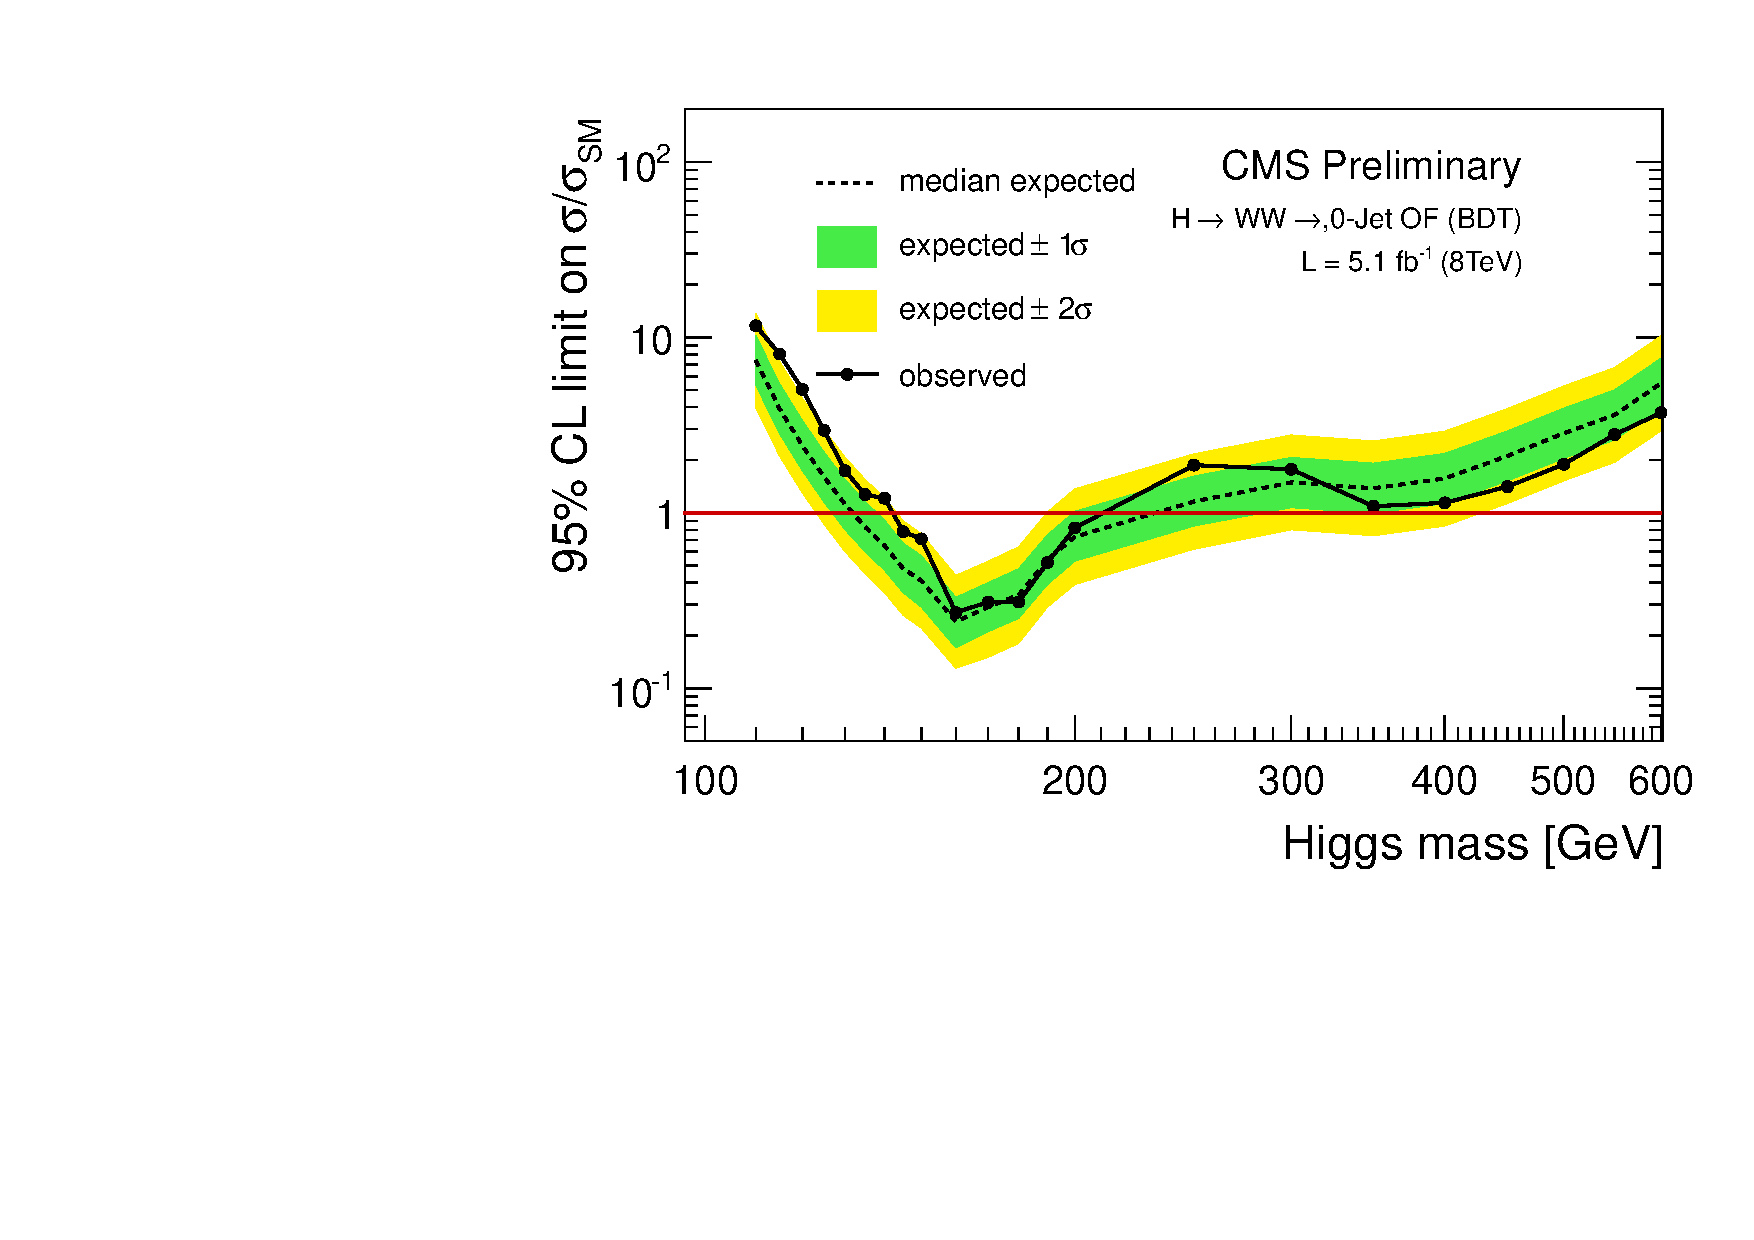
\includegraphics[width=.45\textwidth]{figures/limits_0jof_shape_8TeV-CLs-asymptotic_log.pdf}}
\subfigure[SM Higgs (shape-based) 8 TeV 0-Jet SF ]{
\centering
\label{subfig:sm_shape_8tev_0jsf}
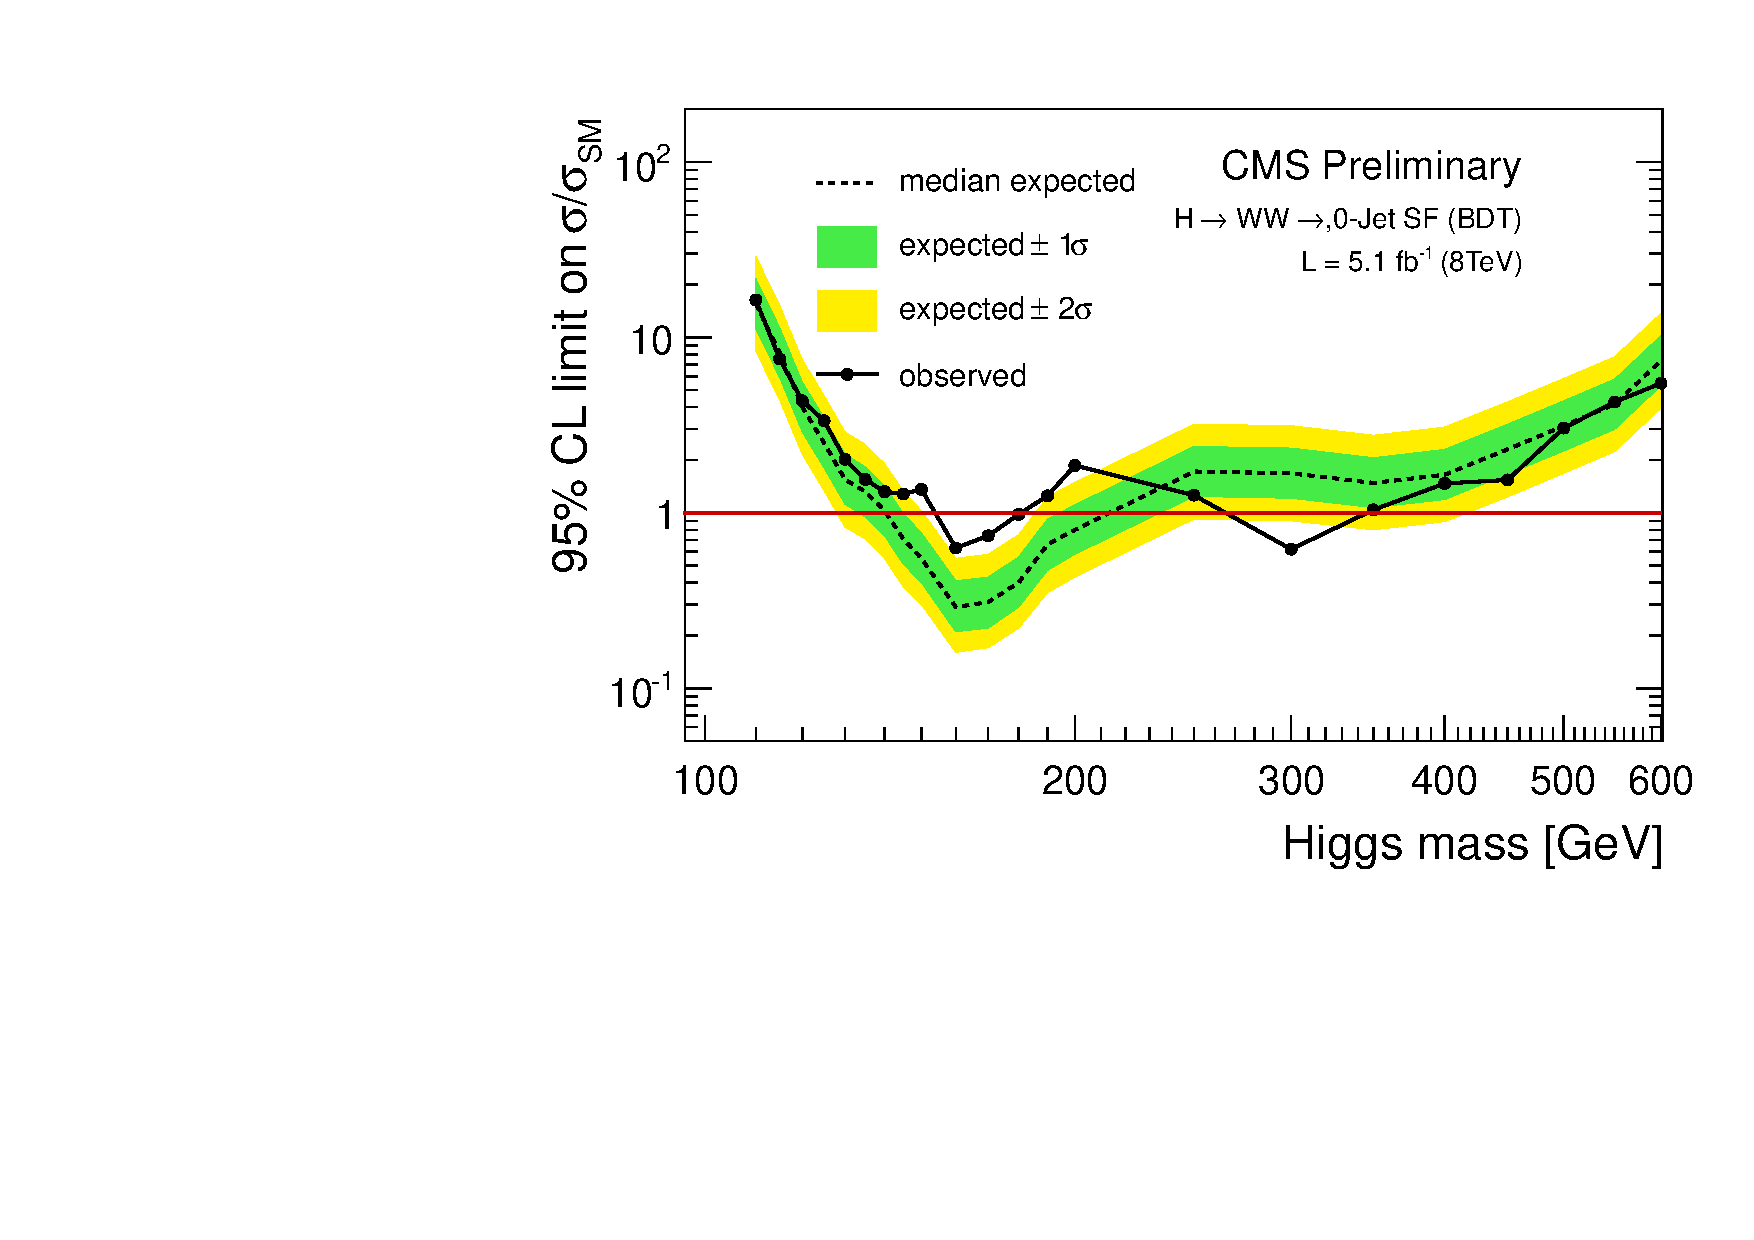
\includegraphics[width=.45\textwidth]{figures/limits_0jsf_shape_8TeV-CLs-asymptotic_log.pdf}} \\
\subfigure[SM Higgs (shape-based) 8 TeV 1-Jet OF ]{
\centering
\label{subfig:sm_shape_8tev_1jof}
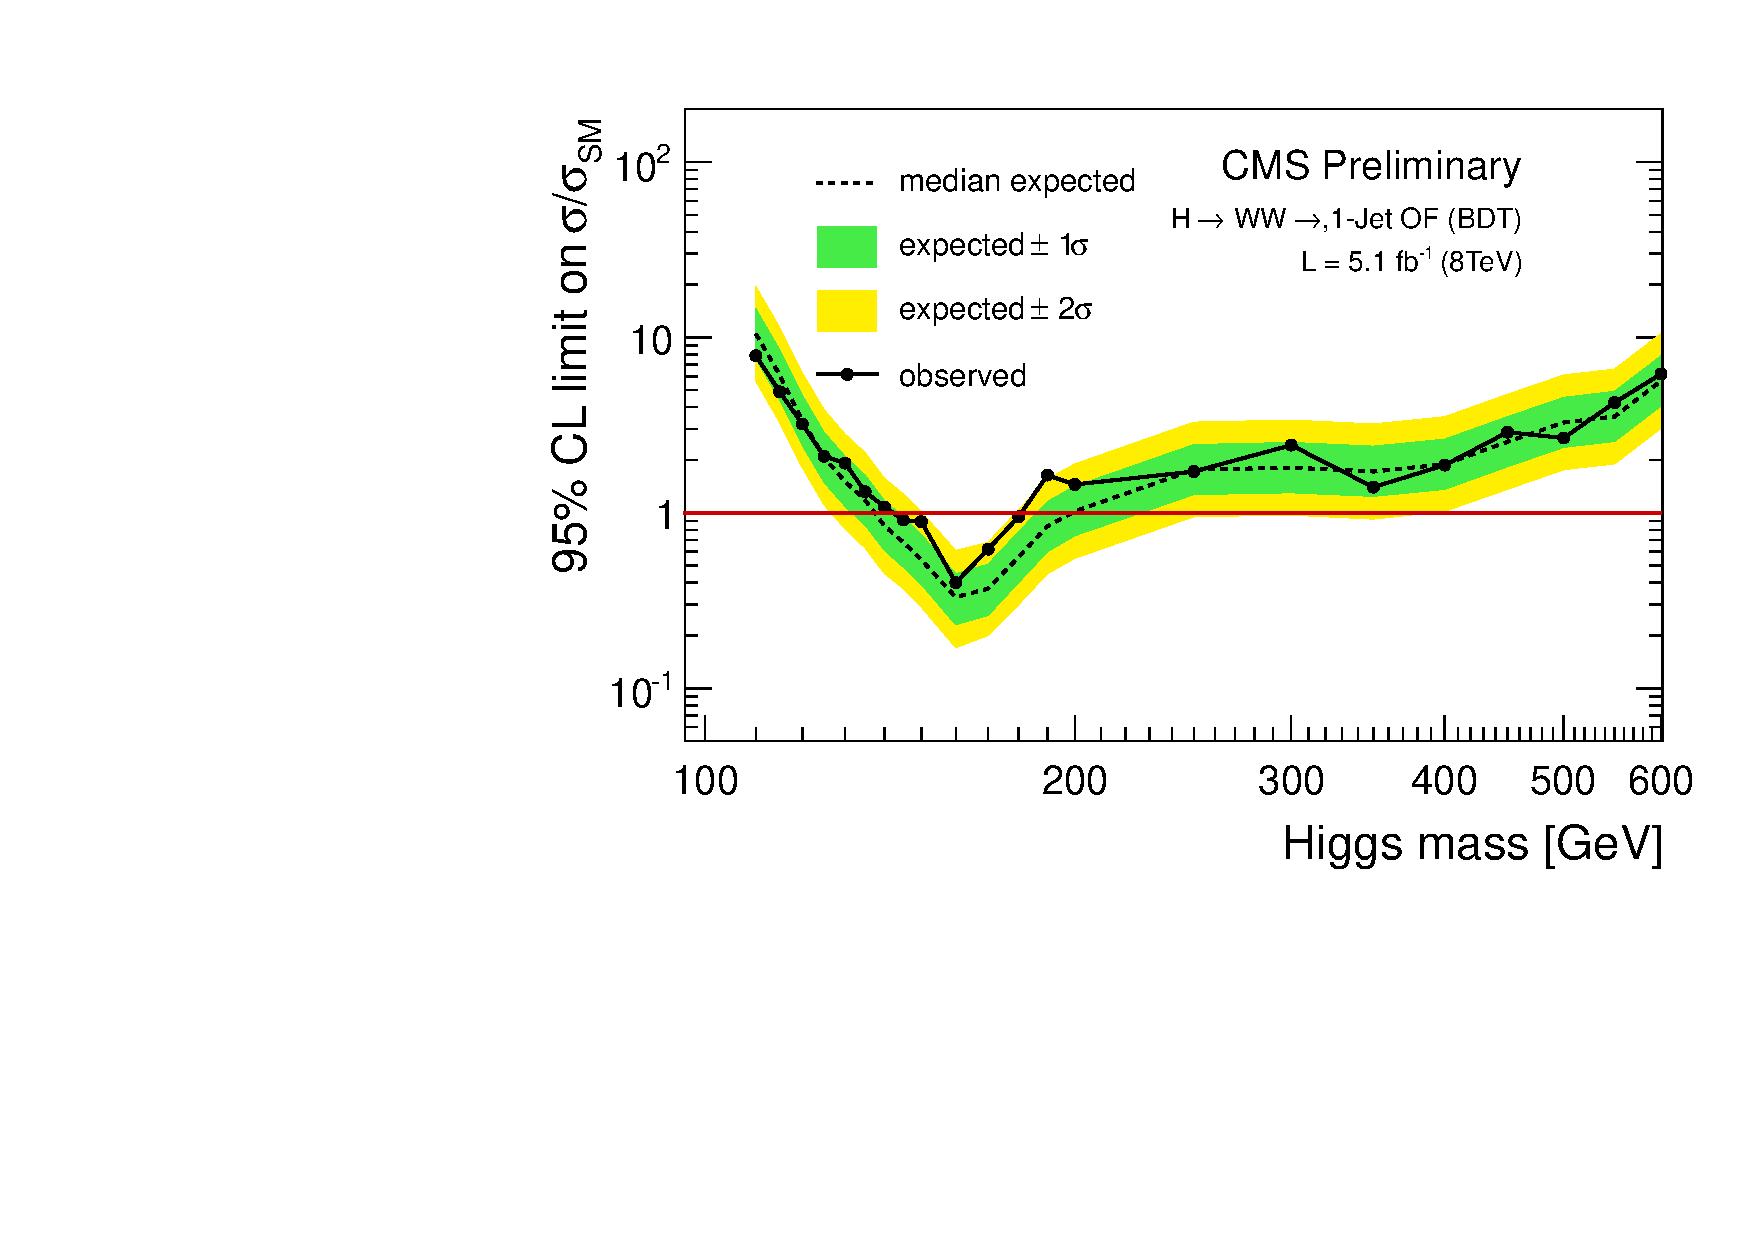
\includegraphics[width=.45\textwidth]{figures/limits_1jof_shape_8TeV-CLs-asymptotic_log.pdf}}
\subfigure[SM Higgs (shape-based) 8 TeV 1-Jet SF ]{
\centering
\label{subfig:sm_shape_8tev_1jsf}
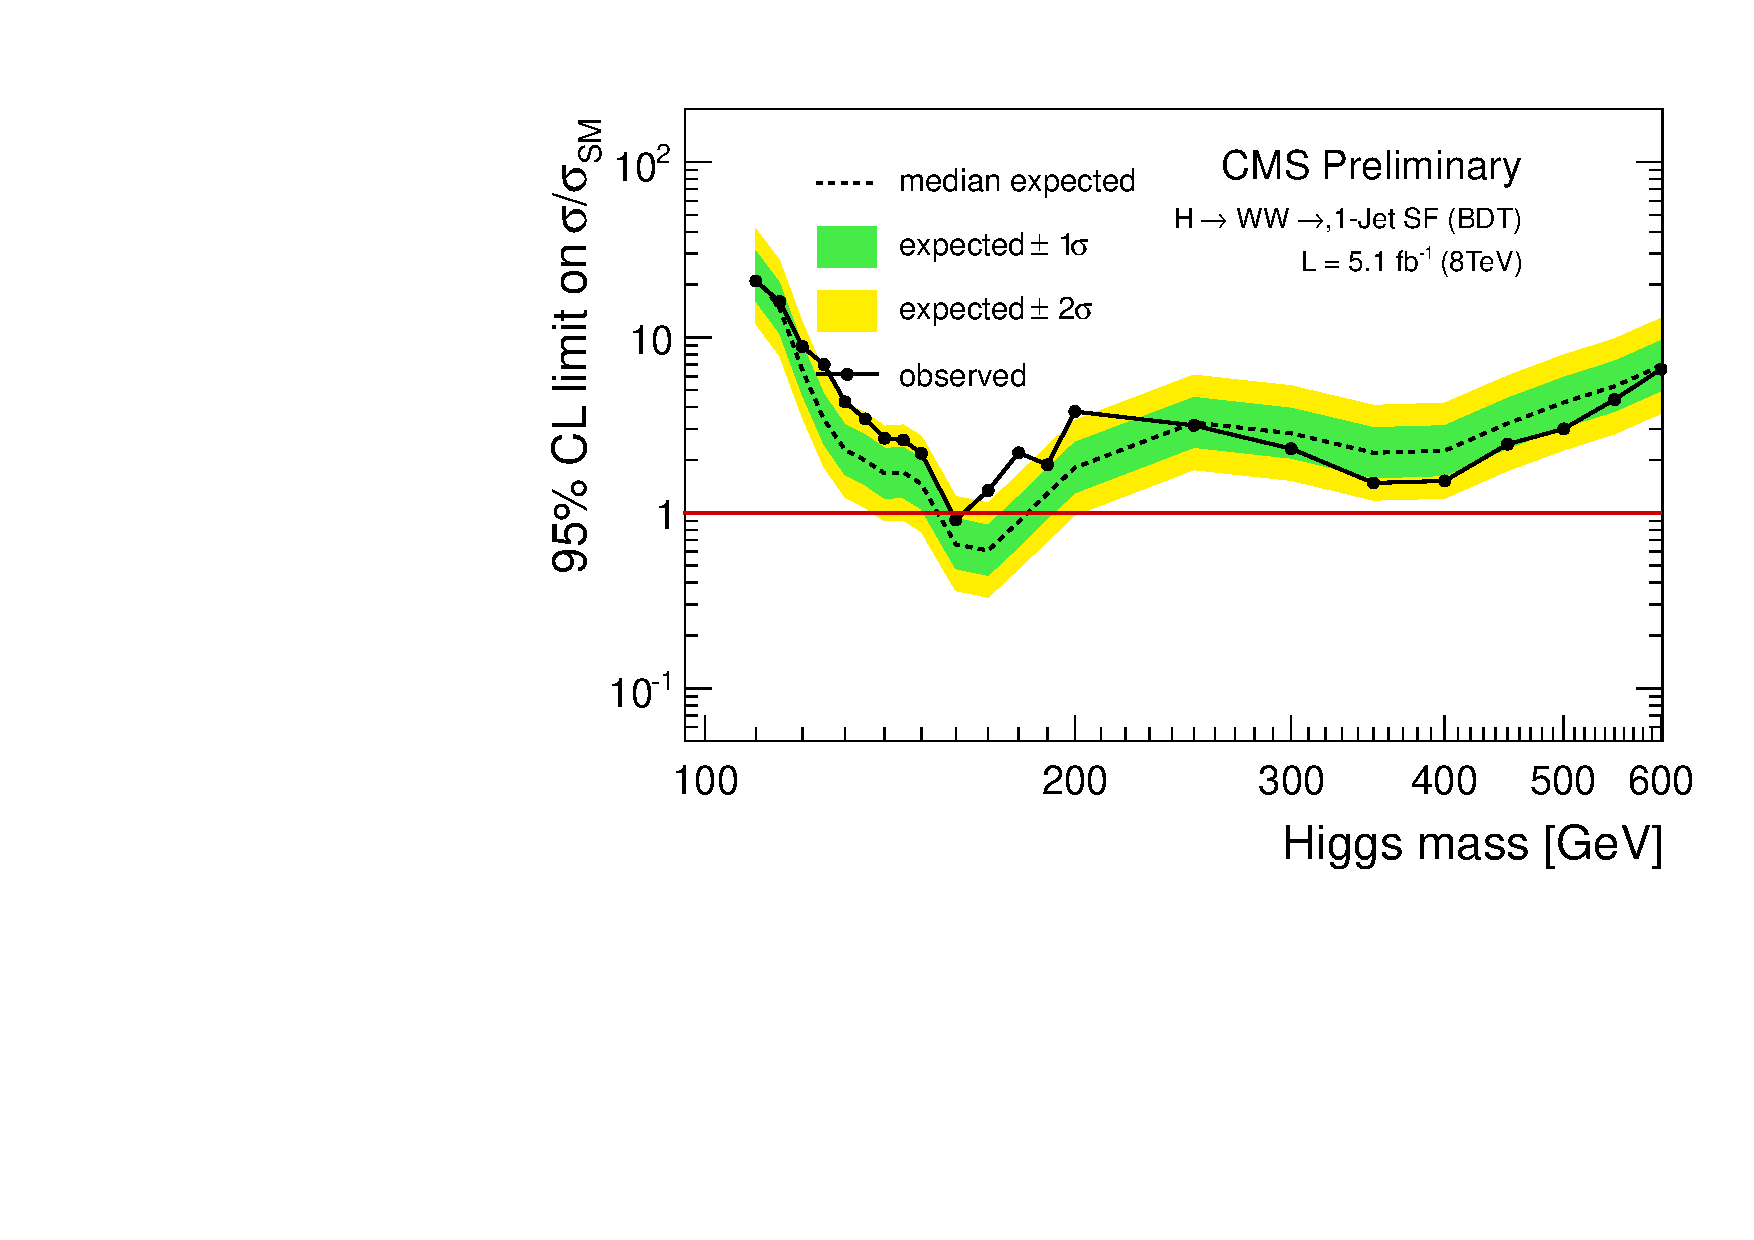
\includegraphics[width=.45\textwidth]{figures/limits_1jsf_shape_8TeV-CLs-asymptotic_log.pdf}} \\
\label{fig:uls_shape_8tev}
\caption{Expected and observed upper limits for SM Higgs using the
  {\bf shape-based} analysis using {\bf 8 TeV data}.}
\end{figure}
%%%%%%%%%%%%%%%%%%%%%%%%%%%%%%%%%%%%%%%%%%%%%%%%%%%%%%%%%%%%
%%%%%%%%%%%%%%%%%%%%%%%%%%%%%%
\begin{table}[hbp!]
\begin{center}
\begin{tabular}{c c c c c}
\hline
\vspace{-3mm} && \\
 Higgs Mass & Observed  & Median expected & Expected range for 68\% & Expected range for 95\%   \\
\vspace{-3mm} && \\
\hline
\multicolumn{5}{c}{0-Jet OF} \\
\hline
110 & 11.65 & 7.38 & [5.32, 10.27] & [3.96, 13.77] \\
115 & 8.04 & 3.92 & [2.82, 5.45] & [2.10, 7.31] \\
120 & 5.06 & 2.42 & [1.74, 3.37] & [1.30, 4.51] \\
125 & 2.95 & 1.60 & [1.15, 2.22] & [0.86, 2.98] \\
130 & 1.74 & 1.12 & [0.80, 1.55] & [0.60, 2.08] \\
135 & 1.27 & 0.83 & [0.60, 1.16] & [0.45, 1.55] \\
140 & 1.21 & 0.65 & [0.47, 0.91] & [0.35, 1.22] \\
145 & 0.78 & 0.48 & [0.35, 0.67] & [0.26, 0.90] \\
150 & 0.71 & 0.41 & [0.29, 0.57] & [0.22, 0.76] \\
160 & 0.27 & 0.24 & [0.17, 0.33] & [0.13, 0.44] \\
170 & 0.31 & 0.29 & [0.21, 0.40] & [0.15, 0.53] \\
180 & 0.31 & 0.34 & [0.25, 0.48] & [0.18, 0.64] \\
190 & 0.52 & 0.54 & [0.39, 0.75] & [0.29, 1.01] \\
200 & 0.82 & 0.73 & [0.53, 1.02] & [0.39, 1.37] \\
250 & 1.87 & 1.16 & [0.84, 1.62] & [0.62, 2.17] \\
300 & 1.77 & 1.49 & [1.07, 2.07] & [0.80, 2.78] \\
350 & 1.09 & 1.38 & [0.99, 1.92] & [0.74, 2.57] \\
400 & 1.14 & 1.57 & [1.13, 2.18] & [0.84, 2.92] \\
450 & 1.41 & 2.11 & [1.52, 2.93] & [1.13, 3.93] \\
500 & 1.89 & 2.84 & [2.04, 3.95] & [1.52, 5.29] \\
550 & 2.79 & 3.61 & [2.60, 5.02] & [1.94, 6.73] \\
600 & 3.72 & 5.47 & [3.94, 7.61] & [2.93, 10.20] \\
\hline
\multicolumn{5}{c}{0-Jet SF} \\
\hline
110 & 16.34 & 15.52 & [11.18, 21.60] & [8.33, 28.96] \\
115 & 7.54 & 8.20 & [5.91, 11.41] & [4.40, 15.30] \\
120 & 4.35 & 4.01 & [2.89, 5.57] & [2.15, 7.47] \\
125 & 3.35 & 2.50 & [1.80, 3.48] & [1.34, 4.66] \\
130 & 2.02 & 1.55 & [1.12, 2.16] & [0.83, 2.89] \\
135 & 1.55 & 1.32 & [0.95, 1.83] & [0.71, 2.46] \\
140 & 1.32 & 1.03 & [0.74, 1.43] & [0.55, 1.91] \\
145 & 1.28 & 0.71 & [0.51, 0.99] & [0.38, 1.33] \\
150 & 1.36 & 0.55 & [0.40, 0.77] & [0.30, 1.03] \\
160 & 0.63 & 0.29 & [0.21, 0.41] & [0.16, 0.55] \\
170 & 0.74 & 0.31 & [0.22, 0.43] & [0.17, 0.58] \\
180 & 0.98 & 0.40 & [0.29, 0.56] & [0.22, 0.75] \\
190 & 1.25 & 0.66 & [0.47, 0.92] & [0.35, 1.23] \\
200 & 1.86 & 0.80 & [0.58, 1.11] & [0.43, 1.49] \\
250 & 1.26 & 1.72 & [1.24, 2.39] & [0.92, 3.20] \\
% 250 & 1.26 & 19.93 & [14.36, 27.73] & [10.69, 37.18] \\ rMax = 30 for exp
300 & 0.62 & 1.68 & [1.21, 2.34] & [0.90, 3.14] \\
350 & 1.04 & 1.48 & [1.07, 2.06] & [0.80, 2.77] \\
400 & 1.47 & 1.65 & [1.19, 2.30] & [0.89, 3.08] \\
% 400 & 1.47 & 18.95 & [13.65, 26.37] & [10.17, 35.35] \\ rMax = 30 for exp
450 & 1.54 & 2.30 & [1.66, 3.20] & [1.23, 4.29] \\
500 & 3.04 & 3.13 & [2.25, 4.35] & [1.68, 5.83] \\
550 & 4.28 & 4.16 & [2.99, 5.78] & [2.23, 7.75] \\
600 & 5.48 & 7.36 & [5.30, 10.24] & [3.95, 13.73] \\

\hline
\end{tabular}
\caption{Expected and observed upper limits for SM Higgs using the
  {\bf shape-based} analysis with \intlumiEightTeV\ of data in the {\bf 0-Jet} final state.}
\label{tab:shapebase_uls_0j}
\end{center}
\end{table}
%%%%%%%%%%%%%%%%%%%%%%%%%%%%%%

%%%%%%%%%%%%%%%%%%%%%%%%%%%%%%%%%%%%%%%%%%%%%%%%%%%%%%%%%%%%
%%%%%%%%%%%%%%%%%%%%%%%%%%%%%%
\begin{table}[hbp!]
\begin{center}
\begin{tabular}{c c c c c  }
\hline
\vspace{-3mm} && \\
 Higgs Mass & Observed  & Median expected & Expected range for 68\% & Expected range for 95\%   \\
\vspace{-3mm} && \\
\hline
\multicolumn{5}{c}{1-Jet OF} \\
\hline
110 & 7.86 & 10.47 & [7.54, 14.56] & [5.62, 19.52] \\
115 & 4.90 & 6.12 & [4.41, 8.51] & [3.28, 11.41] \\
120 & 3.21 & 3.37 & [2.42, 4.68] & [1.81, 6.28] \\
125 & 2.10 & 2.07 & [1.49, 2.88] & [1.11, 3.87] \\
130 & 1.92 & 1.51 & [1.09, 2.10] & [0.81, 2.81] \\
135 & 1.32 & 1.18 & [0.85, 1.64] & [0.63, 2.20] \\
140 & 1.08 & 0.84 & [0.61, 1.17] & [0.45, 1.57] \\
145 & 0.91 & 0.68 & [0.49, 0.95] & [0.37, 1.28] \\
150 & 0.89 & 0.54 & [0.39, 0.75] & [0.29, 1.01] \\
160 & 0.40 & 0.33 & [0.23, 0.45] & [0.17, 0.61] \\
170 & 0.62 & 0.37 & [0.26, 0.51] & [0.20, 0.68] \\
180 & 0.95 & 0.56 & [0.40, 0.78] & [0.30, 1.04] \\
190 & 1.64 & 0.84 & [0.60, 1.16] & [0.45, 1.56] \\
200 & 1.45 & 1.02 & [0.74, 1.42] & [0.55, 1.90] \\
250 & 1.72 & 1.76 & [1.27, 2.45] & [0.95, 3.29] \\
300 & 2.43 & 1.81 & [1.30, 2.52] & [0.97, 3.38] \\
350 & 1.40 & 1.72 & [1.24, 2.40] & [0.92, 3.21] \\
400 & 1.87 & 1.89 & [1.36, 2.63] & [1.02, 3.53] \\
%350 & 1.40 & 19.73 & [14.21, 27.45] & [10.59, 36.80] \\ rMax = 30 for exp
%400 & 1.87 & 20.45 & [14.73, 28.46] & [10.97, 38.15] \\ rMax = 30 for exp
450 & 2.88 & 2.54 & [1.83, 3.53] & [1.36, 4.74] \\
500 & 2.67 & 3.27 & [2.36, 4.55] & [1.76, 6.11] \\
550 & 4.25 & 3.54 & [2.55, 4.93] & [1.90, 6.60] \\
600 & 6.18 & 5.64 & [4.06, 7.85] & [3.03, 10.52] \\
\hline
\multicolumn{5}{c}{1-Jet SF} \\
\hline
110 & 20.96 & 22.26 & [16.04, 30.98] & [11.95, 41.53] \\
115 & 16.00 & 14.67 & [10.57, 20.41] & [7.87, 27.37] \\
120 & 8.87 & 6.53 & [4.70, 9.08] & [3.50, 12.18] \\
125 & 7.00 & 3.39 & [2.45, 4.72] & [1.82, 6.33] \\
130 & 4.29 & 2.29 & [1.65, 3.18] & [1.23, 4.26] \\
135 & 3.43 & 1.99 & [1.44, 2.78] & [1.07, 3.72] \\
140 & 2.66 & 1.68 & [1.21, 2.33] & [0.90, 3.12] \\
145 & 2.60 & 1.70 & [1.22, 2.36] & [0.91, 3.17] \\
150 & 2.18 & 1.46 & [1.05, 2.03] & [0.78, 2.73] \\
160 & 0.91 & 0.66 & [0.48, 0.93] & [0.36, 1.24] \\
170 & 1.34 & 0.61 & [0.44, 0.85] & [0.33, 1.14] \\
180 & 2.20 & 0.89 & [0.64, 1.24] & [0.48, 1.66] \\
190 & 1.88 & 1.29 & [0.93, 1.80] & [0.69, 2.41] \\
200 & 3.78 & 1.81 & [1.30, 2.52] & [0.97, 3.37] \\
250 & 3.56 & 3.49 & [2.52, 4.86] & [1.87, 6.51] \\
%250 & 3.56 & 27.33 & [19.69, 38.03] & [14.67, 50.98] \\ rMax = 30
300 & 2.32 & 2.84 & [2.05, 3.95] & [1.53, 5.30] \\
350 & 1.48 & 2.20 & [1.58, 3.06] & [1.18, 4.10] \\
400 & 1.52 & 2.26 & [1.63, 3.14] & [1.21, 4.22] \\
450 & 2.46 & 3.23 & [2.33, 4.50] & [1.74, 6.03] \\
500 & 3.01 & 4.26 & [3.07, 5.92] & [2.28, 7.94] \\
550 & 4.42 & 5.26 & [3.79, 7.32] & [2.82, 9.81] \\
600 & 6.59 & 6.88 & [4.96, 9.58] & [3.69, 12.84] \\
\hline
\end{tabular}
\caption{Expected and observed upper limits for SM Higgs using the
  {\bf shape-based} analysis with \intlumiEightTeV\ of data in the {\bf 1-Jet} final state.}
\label{tab:shapebase_uls_1j}
\end{center}
\end{table}
%%%%%%%%%%%%%%%%%%%%%%%%%%%%%%
